\documentclass{amsart}
\usepackage{graphicx,amsfonts,amsthm,amsmath,amssymb,enumerate,enumitem,xcolor,commath,hyperref} % Required for inserting images
\usepackage{geometry}[margin=0.75in]
\usepackage{biblatex}[sorting=none]

\title{An Introduction to Computational Stochastic PDEs\\ Exercises: Chapter 1}
\author{Chris DuPre }
\date{April 2024}

\theoremstyle{plain}
\newtheorem{thm}{Theorem}[section]
\newtheorem{lem}[thm]{Lemma}
\newtheorem{prop}[thm]{Proposition}
\newtheorem*{cor}{Corollary}

\theoremstyle{definition}
\newtheorem{defn}{Definition}[section]
\newtheorem{conj}{Conjecture}[section]
\newtheorem{exmp}{Example}[section]
\newtheorem{exer}{Exercise}[section]

\newcommand{\R}{\mathbb{R}}
\newcommand{\C}{\mathbb{C}}
\newcommand{\Z}{\mathbb{Z}}
\newcommand{\Q}{\mathbb{Q}}
\newcommand{\N}{\mathbb{N}}
\newcommand{\Hil}{\mathcal{H}}
\newcommand{\E}{\mathcal{E}}
\DeclareMathOperator{\csch}{csch}
\DeclareMathOperator{\sech}{sech}

\newcommand{\tcr}[1]{\textcolor{red}{#1}}

\bibliography{Ref}

\begin{document}

\maketitle
\setcounter{section}{1}
\begin{exer}
For a bounded domain $D$, prove that $C\left(\overline{D}\right)$ is complete with respect to the supremum
norm $\|u\|_{\infty} = \sup_{x \in D} \abs{u(x)}$. By constructing a suitable Cauchy sequence, show that
$C\left(\overline{D}\right)$ is not complete with respect to the $L^{2}(D)$ norm. 
\end{exer}
\begin{proof}
    First, note that $\overline{D}$ is bounded as $D$ is bounded. Thus by Heine-Borel, $\overline{D}$ is compact. As continuous functions achieve their supremeum on compact sets, each $f_k$ is bounded. Define $M_n := \sup_{y\in \overline{D}} f(y)$. We first claim that $f_k$ as a sequence is uniformly bounded. To see this, note that as $f_k$ is Cauchy, there exists an $N$ such that for all $m,l\geq N$ we have that $\|f_m-f_l\|_{\infty} < 1.$ We thus have that $\sup_{y\in \overline{D}} \abs{f_l(y)} \leq M_N + 1.$ We thus have that $\sup_{k\in \N, x\in \overline{D}}\abs{f_k(x)} \leq \max\left\{\{M_k\}_{k=1}^{N}\right\}+1.$
    \par 
    As these are uniformly bounded, in particular for every $y\in \overline{D}$, we have that $f_k(y)$ is bounded and Cauchy. As $\R$ is complete, it must converge. For every $x\in \R$, define
    $$f(x) = \lim_{k\to \infty} f_k(x).$$
    We claim that $\lim_{k\to \infty} \sup_{y\in D} \abs{f_k(y)-f(y)} = 0$, (we do not use the norm as a-priori we do not know this function is continuous). As $\abs{\cdot}$ and subtraction are continuous, it is clear that for every $y \in \overline{D}$ that
    $$\abs{f_{k}(y)-f(y)} \leq\lim_{m\to \infty}\abs{f_{k}(y)-f_{m}(y)} \leq \limsup_{m\to \infty} \|f_k -f_m\|_{\infty}.$$
    As the right hand side is independent of $y$, we may take the supremum over the right hand side. For all $\varepsilon > 0$, there exists an $N$ such that the right hand side is less than $\varepsilon$ if $k=N$. As $\varepsilon$ is arbitrary, it is clear that 
    $$lim_{k\to \infty} \sup_{y\in D} \abs{f_k(y)-f(y)} = 0.$$
    \par We now claim that $f$ is continuous. To see this, note
    $$\abs{f(x)-f(y)}\leq \abs{f(x)-f_k(x)}+\abs{f_k(x)-f_k(y)}+\abs{f_k(y)-f(y)}.$$
    By the previous statement, there exists a $k$ such that the first and last terms are less than $\varepsilon/3$ for all $x,y\in\overline{D}.$ As $f_k$ is then continuous, there exists $\delta > 0$ such that if the distance between $x,y$ is less than $\delta$ we have that the middle term is less than $\varepsilon/3$. Thus $f$ is continuous.
    \par As a counter example for $L^2$, consider
    $$f_k(x) = \begin{cases}
        0 & -2\leq x \leq -1-\frac{1}{k}\\
        \frac{k(x+1)+1}{2}& \abs{x+1}\leq \frac{1}{k}\\
        1 & \abs{x}\leq 1-\frac{1}{k}\\
        \frac{k(1-x)+1}{2}& \abs{x-1}\leq \frac{1}{k}\\
        0 & 1+\frac{1}{k}\leq x\leq 2
    \end{cases}$$
    \begin{figure}[h!]
        \centering
        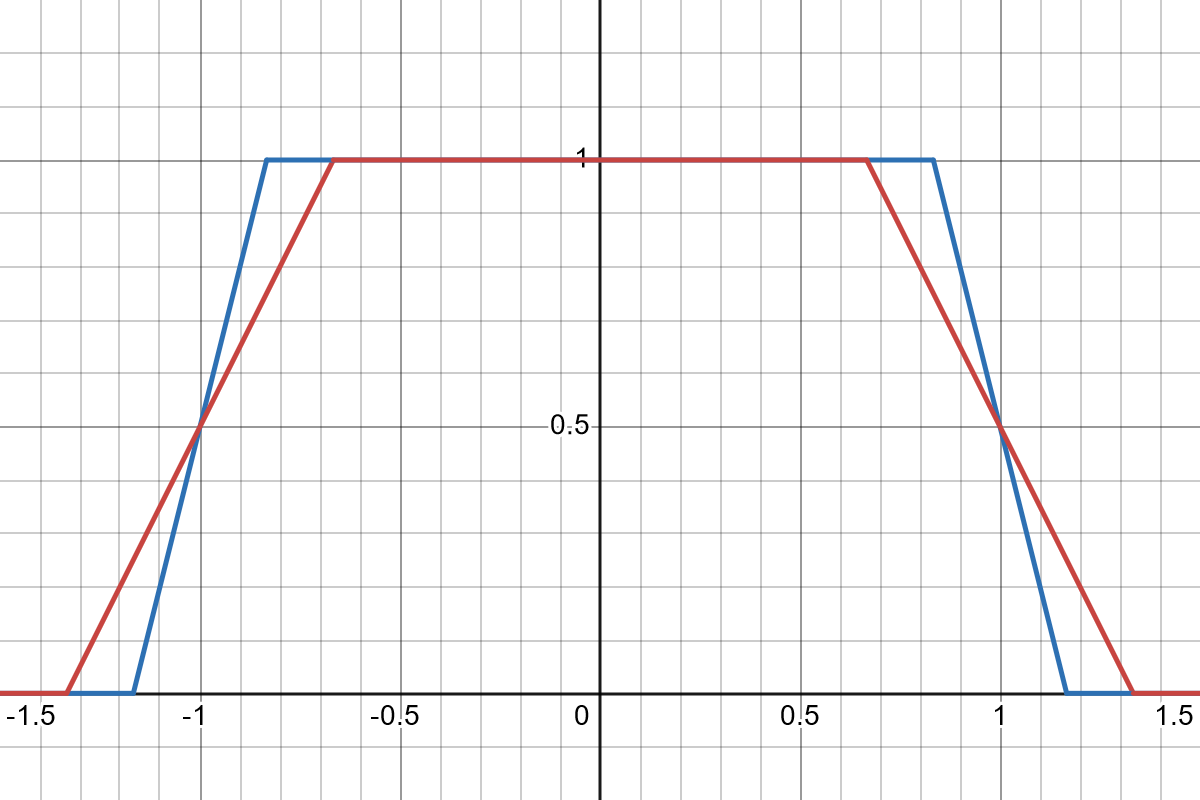
\includegraphics[width=0.5\linewidth]{Exercises/Chapter 1/Photos/Problem1Counter.png}
        \caption{Depiction of counter example family. Red is $k=3$. Blue is $k=7$.}
        \label{fig:Problem_1_counter}
    \end{figure}
    This family is clearly continuous on $[-2,2].$ It is also clearly Cauchy, as in particular
    $$\|f_k - f_m\|_{L^2} \leq \frac{2}{\min_{m,k}}.$$
    However, this sequence converges to $\mathbf{1}_{[-1,1]}$ which is not continuous and therefore not in the space. Thus we have a Cauchy sequence which does not converge and the space is not complete
\end{proof}

\begin{exer}
    Let $\left(X,\mathcal{F},\mu \right)$ be a complete measure space, $Y$ be a Banach space, and $f : X \to Y$ a measurable function. Show that $f = g$ a.s. implies that g is measurable. Give an example to show that the completeness assumption on the measure space is necessary.
\end{exer}
\begin{proof}
Note that $f= g$ a.s. implies that there exists a measurable null set $N$ such that $f=g$ on $N^C$. Let $B$ be measurable and consider $g^{-1}(B).$ Then clearly $g^{-1}(B) = g^{-1}(B)\cap N \cup g^{-1}(B) \cap N^C = g^{-1}(B)\cap N \cup f^{-1}(B) \cap N^C.$ By completeness, $g^{-1}(B)\cap N$ is measurable. Thus $g^{-1}(B)$ is a finite union of measureable sets and is thus measureable. 
\par To see that completeness is neccesary. Consider $X = \{1,2,3\}, \mathcal{F} = \{\empty,\{1\},\{2,3\},\{1,2,3\}\}$ with $\mu\left(\{1\}\right) = 1, \mu\left(\{2\}\right)=\mu\left(\{3\}\right).$ Let $f$ be defined as $f(1) = f(2) = 0, f(3) = 0$ and $g(1)=g(3) = 1, g(2) = 0$. Note that $f = g$ a.s. with $N = \{2,3\}$ and $f$ is measureable but $g$ is not.  
\end{proof}

$$\int_{X} \|u(x)\|_{Y} dx < \infty.$$
\begin{exer}
   Using Definition 1.2.1 in \cite{lord2014introduction}, prove that if $u:X\to Y$ is integrable then 
        $$\int_{X} \|u(x)\|_{Y} dx < \infty.$$
\end{exer}
\begin{proof}
    Note that 
    \begin{align*}
        \int_{X} \|u(x)\|_{Y} dx &\leq \int_{X} \|u(x)-u_k(x)\|_{Y} dx + \int_{X} \|u_k(x)\|_{Y} dx \\
        & = \int_{X} \lim_{m\to \infty} \|u_m(x)-u_k(x)\|_{Y} dx + \int_{X} \|u_k(x)\|_{Y} dx \\
        & \leq \liminf_{m}\int_{X} \|u_m(x)-u_k(x)\|_{Y} dx+ \int_{X} \|u_k(x)\|_{Y} dx.
    \end{align*}
    The last inequality follows by Fatou's lemma. 
    For $k$ sufficiently large , the first term is bounded by $1$ by Definition 1.2.1. By the definition of simple functions, the second is also bounded. Thus the term on the left is bounded as well.
\end{proof}

\begin{exer}
    \begin{enumerate}[label=\alph*.]
        \item If $u:\R\to\R$ is measurable, define simple functions $u_n$ such that $u_n(x) \to u(x)$ for all $x\in\R.$
        \item If $G\in C\left(\R\times \R\right)$, define simple functions of the form
        $$\sum_{j,k=1}^{N} G(x_j,x_k)\mathbf{1}_{\mathcal{F}_j}\mathbf{1}_{\mathcal{F}_k}$$
        for $x_j\in\R, F_j \in \mathcal{B}\left(\R\right)$, such that $G_j\to G$ point-wise as $N\to \infty.$
    \end{enumerate}
\end{exer}
\begin{proof}
    \begin{enumerate}[label=\alph*.]
        \item Define $\mathcal{F}_{j}^{n} = u^{-1}\left(\left[\frac{j}{n},\frac{j+1}{n}\right)\right)\cap\left[-n,n\right], -n^2 \leq j \leq n^2$ and define:
        $$u_n(x) = \sum_{j=-n^2}^{n^2} \frac{j}{n}\mathbf{1}_{\mathcal{F}_{j}^{n}}.$$
        It is clear this function is simple as each set is clearly measurable and $\mu\left(\mathcal{F}_j^n\right)\leq 2n$. Consider $x\in \R$. Then for $n\geq \lceil \abs{x}\rceil$, we have that $\abs{u(x)-u_{n}(x)}\leq \frac{1}{n}$ and thus it converges point-wise.
        \item Let $F_j^n = \left[\frac{j}{n},\frac{j+1}{n}\right), -n^2 \leq j \leq n^2$ and define 
        $$G_n(x,y) = \sum_{j=-n^2}^{n^2}\sum_{k=-n^2}^{n^2} G\left(\frac{j+1/2}{n},\frac{k+1/2}{n}\right)\mathbf{1}_{F_j^n}(x)\mathbf{1}_{F_k^n}(y).$$
        To see point-wise convergence, fix $(x,y) \in \R\times\R.$ As $G$ is continuous, for every $\varepsilon>0$ there exists an $N$ large enough such that if $(x_1,y_1)$ and $(x_2,y_2)$ are less than $\frac{1}{\sqrt{2}N}$ apart then $\abs{G(x_1,y_1)-G(x_2,y_2)}\leq \varepsilon$. For each such $\varepsilon$, pick $n \geq \max\{\lceil \abs{x}\rceil, \lceil \abs{y} \rceil, N\}.$ We then claim that $\abs{G_n(x,y)-G(x,y)}\leq \varepsilon.$ This is because every point is shifted to another point at most $\frac{1}{\sqrt{2}N}$ away, which is chose so that the difference is less than $\varepsilon.$
    \end{enumerate}
\end{proof}

\begin{exer}
    Give an example of a Lebesgue integrable function $u : R \to R$ that is not Riemann integrable.
\end{exer}
\begin{proof}
Let $f$ be defined as 
$$f(x) = \begin{cases}
    1 & x\in \Q\\
    0& \text{else}.
\end{cases}$$
It is clear that $f$ is Lebesgue integrable and that in fact $\int \abs{f}dx = 0.$ However, we claim $f$ is not integrable. This is because the function is not of finite variation. This can be seen by taking the sequence of partitions $\pi_n=\cup_{j=0}^{n-1} \left[\frac{j}{n}, \frac{j+\pi/4}{n}\right) \cup \left[\frac{j+\pi/4}{n},\frac{j+1}{n}\right)$. The variation at each level in this partition is clearly $2n$ and is thus unbounded. 
\end{proof}

\begin{exer}
    By introducing a measure on $\Z$, show that 
    $$\lim_{n\to \infty} \sum_{j\in \Z} u_{n,j} \to \sum_{j\in \Z} u_{j}$$
    if $\lim_{n\to\infty} u_{n,j} = u_{j}$ and such that $\abs{u_{n,j}} \leq U_{j}$ for some $U_j$ such that $\sum_{j\in\Z} U_j < \infty.$
\end{exer}
\begin{proof}
    Take the counting measure, where $c(A) = \abs{A}$ where $A\subset \Z$ and $\abs{A}$ is the sets cardinality. The result now follows by Lebesgue dominated convergence theorem. 
\end{proof}

\begin{exer}
    Evaluate
    $$\int_{0}^{b}\int_{0}^a f(x,y) dx dy , \int_{0}^{a}\int_{0}^{b} f(x,y) dy dx.$$
    Where 
    $$f(x,y) = \begin{cases}
        \frac{xy\left(y^2-x^2\right)}{\left(x^2+y^2\right)^3}  & (x,y) \neq (0,0)\\
        0 & (x,y) = (0,0).
    \end{cases}$$
    Why does Fubini's theorem \textit{not} apply?
\end{exer}
\begin{proof}
    For the computations, we have
    \begin{align*}
        \int_{0}^{b}\int_{0}^a f(x,y) dx dy &= \int_{0}^b \left[\frac{1}{2}\frac{x^2y}{\left(x^2+y^2\right)^2}\right]_{x=0}^{x=a} dy\\
        &= \frac{1}{2}\int_{0}^b \frac{a^2 y}{\left(a^2+y^2\right)^2} dy\\
        &= \frac{-1}{4}\left[\frac{a^2}{a^2+y^2}\right]_{y=0}^{y=b}\\
        &= \frac{1}{4}\left[1-\frac{a^2}{a^2+b^2}\right]=\frac{b^2}{4\left(a^2+b^2\right)}\\
        \int_{0}^{a}\int_{0}^b f(x,y) dy dx &= \int_{0}^b \left[\frac{-1}{2}\frac{xy^2}{\left(x^2+y^2\right)^2}\right]_{y=0}^{y=b} dx\\
        &= \frac{-1}{2}\int_{0}^a \frac{b^2 x}{\left(b^2+x^2\right)^2} dx\\
        &= \frac{-1}{4}\left[\frac{b^2}{b^2+x^2}\right]_{x=0}^{x=a}\\
        &= \frac{1}{4}\left[1-\frac{b^2}{a^2+b^2}\right]=\frac{a^2}{4\left(a^2+b^2\right)}.
    \end{align*}
    The reason Fubini's does not imply is it is not absolutely integrable. In fact, in polar coordinates the function takes the form $f(r,\theta) = \frac{\sin(4\theta)}{4r^2}.$ Therefore, any cone about $\theta=\pi/8+n*\pi/4, n\in\Z$ will show exactly this problem.
\end{proof}

\begin{exer}
    Using Fubini's theorem, prove that 
    $$\frac{1}{\sqrt{2\pi}}\int_{-\infty}^{\infty} e^{-\frac{x^2}{2}}dx = 1.$$
\end{exer}
\begin{proof}
Formally multiplying this integral with itself gives 
$$\frac{1}{2\pi}\int_{\R^2} e^{-\frac{x^2+y^2}{2}} dx dy$$.
As this function is non negative, we can show that if it is integrable, it is absolutely integrable. Transferring to polar coordinates gives
$$\frac{1}{2\pi}\int_{r=0}^{\infty}\int_{\theta=0}^{2\pi} e^{-\frac{r^2}{2}} r dr d\theta = 1.$$
Thus the function is integrable and its square is 1. As the function is non-negative, the integral must be 1.   
\end{proof}

\begin{exer}
    For $f\in C^1\left( [0,1] \right)$ and $p\geq 1$, prove that
    $$\left(\int_0^1 \abs{f(x)} dx\right)^p \leq \int_0^1 \abs{f(x)}^p dx$$
    This is a version of Jensen's inequality. For $a<b$, show that $L^q (a,b)\subset L^p(a,b)$ for $1\laq p \leq q.$
\end{exer}
\begin{proof}
By H\"older's inequality
$$\int_0^1 \abs{f(x)}\times 1 dx \leq \left(\int_0^1 \abs{f(x)}^p\right)^{1/p} \left( \int_0^1 dx\right)^{1/q} = \left(\int_0^1 \abs{f(x)}^p\right)^{1/p}.$$ 
Raise both sides to the $p$ power to obtain the desired inequality. Let $1\leq p\leq q$. Let $r = \frac{q}{p}.$ Applying the above procedure with $r$ gives
$$\int_a^b \abs{f(x)}^p\times 1 dx \leq \left(\int_a^b \abs{f(x)}^q\right)^{1/r} \left( \int_a^b dx\right)^{1-1/r} = \left(\int_0^1 \abs{f(x)}^p\right)^{p/q} \left(b-a\right)^{\frac{q-p}{q}}.$$
Raising both side to $1/p$ bounds the left hand side by a constant multiple of the right hand side. Thus if $f\in L^q$, $f\in L^p$ or $L^q([a,b]) \subset L^p([a,b]).$
\end{proof}

\begin{exer}
    On a real Hilbert space $H$, prove the Cauchy–Schwarz inequality $\abs{\langle u, v\rangle}\leq \|u\|\|v\|$ for $u,v\in H.$
\end{exer}
\begin{proof}
If both $u = 0$ and $v= 0$, the statment is trivial. Assume without loss $v \neq 0$. Consider $f(\alpha) = \|u+\alpha v\|^2.$ Taking the derivative with respect to $\alpha$ gives $\frac{df}{d\alpha} = -2\langle u,v\rangle + 2\alpha \|v\|_{2}^{2}.$ Seeking an critical point gives $\alpha = \frac{\langle u,v\rangle}{\|v\|^2}.$ Evaluating at this critical point gives 
$$0\leq \|u+\alpha v\|^2 = \|u\|^2 - 2\frac{\langle u,v\rangle^2}{\|v\|^2}+\frac{\langle u,v\rangle^2}{\|v\|^2} = \|u\|^2 - \frac{\langle u,v\rangle^2}{\|v\|^2}.$$
Rearranging and taking the square root of both sides gives the Cauchy-Schwarz inequality.
\end{proof}

\begin{exer}
    Prove that $(1.12)$ is the weak derivative of $(1.11)$  (by showing that $(1.13)$ holds) (Equations on p. 12 of \cite{lord2014introduction}) and that $\mathcal{D}u$ does not have a weak derivative in the set of measurable functions $u:\R\to\R.$
\end{exer}
\begin{proof}
Assume by density that $\phi \in C^\infty_c(\R).$
    \begin{align*}
        \int_\R \mathcal{D}u(x) \phi(x) dx &= \int_{0}^\infty \phi(x) dx \\
        &= -\int_{0}^\infty x\phi'(x)dx = -\int_{\R} u(x)\phi'(x) dx. 
    \end{align*}
\end{proof}

\begin{exer}
    \begin{enumerate}[label=\alph*.]
        \item Let $u(r) = \log\left(\abs{\log(r)}\right)$ for $r> 0$. Sketch a graph of $u(r)$ and $u'(r).$ Show that $u\in L^2\left(\left[0,\frac{1}{2}\right]\right)$ but $u\not \in C\left(\left[0,\frac{1}{2}\right]\right)$ and $u' \not \in L^2\left(\left[0,\frac{1}{2}\right]\right)$
        \item Let $u(\mathbf{x}) = \log\left(\log(r)\right), r=\|x\|_{2}$ and $D = \left\{\mathbf{x} \in \R^2 \vert \|x\|_{2} \leq \frac{1}{2}\right\}.$ Show that $u$ has a well-defined weak derivative $D_i u \in L^2(D)$ for $i=1,2.$ Hence, show that $u\in H^1(D)$ and $u\not \in C\left(\overline{D}\right).$
    \end{enumerate}
\end{exer}
\begin{proof}
    \begin{enumerate}[label=\alph*.]
        \item By direct computation $u'(r) = \frac{1}{r\log(r)}$. A sketch of two graphs is shown below.
        \begin{figure}[h!]
            \centering
            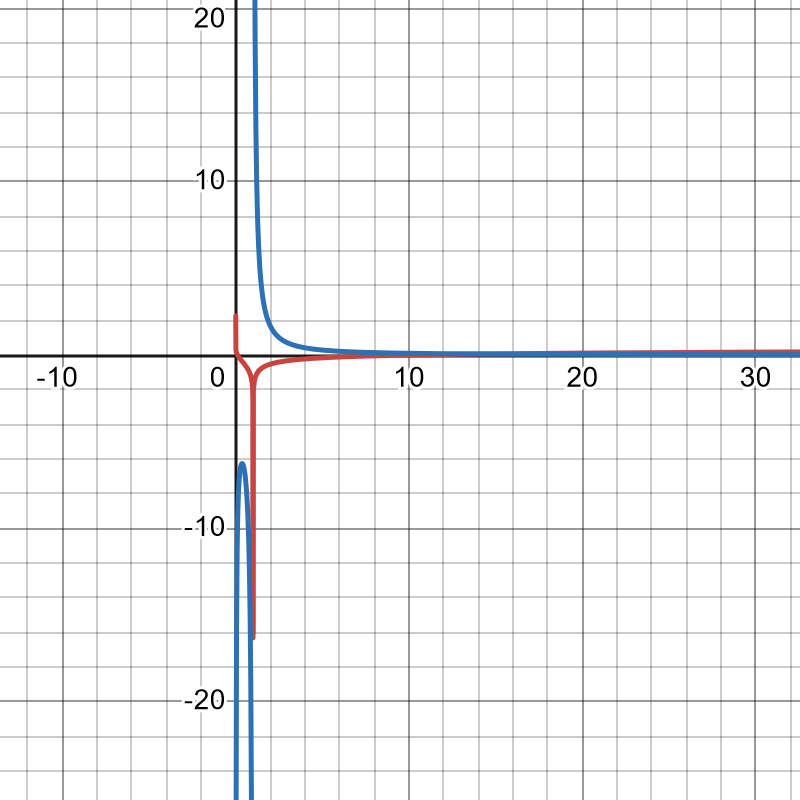
\includegraphics[width=0.5\linewidth]{Exercises/Chapter 1/Photos/Problem12A.png}
            \caption{Sketch of \textcolor{red}{$u(r)$} and \textcolor{blue}{$u'(r)$}.}
            \label{fig:12a}
        \end{figure}
        To see $u\in L^2([0,1/2])$ we can compute:
        $$\int_0^{1/2} \log\left(-\log x\right) dx = \int_{2}^{\infty} \frac{\log\left(\log u\right)^2}{u^{1/2}}\frac{1}{u^{3/2}}du.$$ Notice that for all $x\geq 0$ we have that $\log(x) < x$ and that $\log(x)$ is increasing so $\log(\log(x))^2 \leq \log(x)^2.$ 
        Further, we have that $x^{1/2} > \log(x)^2$ for all $x\geq 1$. Thus we have that
        \begin{align*}
            \int_0^{1/2} \log\left(-\log x\right) dx &= \int_{2}^{\infty} \frac{\log\left(\log u\right)}{u^{1/2}}\frac{1}{u^{3/2}}du\\
            &\leq \int_2^\infty \frac{1}{u^{3/2}} du = \left[\frac{-2}{u^{1/2}}\right]_{u=2}^{u=\infty} =  \frac{1}{\sqrt{2}} < \infty.
        \end{align*}
        Thus $u\in L^2([0,1/2]).$ u does not admit a continuous extension as in particular $\lim_{n\to\infty} \abs{u\left(\frac{1}{n}\right)} = \infty$ so $u(0)$ cannot be defined. $u'(r)\not \in L^2([0,1/2])$ as by direct computation:
        $$\int_{0}^{1/2} \frac{1}{r^2\log(r)^2} dr \geq \int_{0}^{1/2} \frac{1}{r\log(r)^2} \frac{1}{r}dr.$$
        Notice that for all $x\leq 1$ we have that
        $\frac{1}{x\log(x)^2} \geq 1.$ Thus we have that 
        \begin{align*}
            \int_{0}^{1/2} \frac{1}{r^2\log(r)^2} dr &= \int_{0}^{1/2} \frac{1}{r\log(r)^2} \frac{1}{r}dr\\
            &\geq \int_{0}^{1/2}  \frac{1}{r}dr.
        \end{align*}
        But the last integral diverges. Therefore $u'\not \in L^2([0,1/2])$
        \item It is clear that $u\not \in C\left(\overline{D}\right)$ as $u(r)\not \in C\left(\left[0,\frac{1}{2}\right)\right)$ and the function is radial. To see that the function admits a weak-derivative, notice that 
        \begin{align*}
            \int_{D} u(\mathbf{x})\nabla \phi\left(\mathbf{x}\right) d\mathbf{x} &= \left[\int_{0}^{1/2}\int_{0}^{2\pi}  r u(r) \frac{\partial \phi(r,\theta)}{\partial r} d\theta dr\right] \mathbf{e}_r + \left[\int_{0}^{1/2}\int_{0}^{2\pi} u(r) \frac{\partial \phi(r,\theta)}{\partial \thetat} d\theta dr \right]\mathbf{e}_\theta\\
            &= \left[\int_{0}^{2\pi} \left[\left[ru(r)\phi(r,\theta)\right]_{r=0}^{1/2}-\int_{0}^{1/2} \left(ru'(r)+u(r)\right)\phi(r,\theta)\right]d\theta\right] \mathbf{e}_r \\
            &+ \left[\int_{0}^{1/2} u(r) \left[\phi(r,\theta)\right]_{\theta=0}^{\theta=2\pi} dr \right]\mathbf{e}_\theta\\
            &= \int_{0}^{2\pi} \frac{u\left(\frac{1}{2}\right)\phi\left(\frac{1}{2},\theta\right)}{2}d\theta \mathbf{e}_r - \left[\int_{0}^{\frac{1}{2}} \int_{0}^{2\pi} \left(u'(r)+\frac{u(r)}{r}\right)\phi(r,\theta) r d\theta dr \right]\mathbf{e}_r.
        \end{align*}
        Thus if we can show that $ru'(r) + u(r) \in L^2\left(\left[0,\frac{1}{2}\right]\right)$, then the weak derivative is given by $\nabla u\left(\mathbf{x}\right) = \left[\frac{u\left(r\right)}{r} + u'(r) \right] e_r.$ We have already show $u(r) \in L^2\left(\left[0,\frac{1}{2}\right]\right)$. For the second term, notice
        $$\int_{0}^{1/2} r^2 u'(r)^2 dr = \int_{0}^{1/2} \frac{1}{\log(r)^2} dr \leq \int_{0}^{1/2} \frac{1}{\log(2)^2} dr = \frac{1}{2\log(2)^2} < \infty. $$
        Thus $u\left(\mathbf{x}\right)\in H^1(D).$
    \end{enumerate}
\end{proof}

\begin{exer}
For  $l >0$ and $u \in C^{n+1}\left(\left[-l,l\right]\right)$, show that there exists a polynomial $p$ of degree at most $n$ such that
$$\|u-p\|_{L^2\left(\left[-l,l\right]\right)} \leq \frac{1}{\left(n+1\right)!}\|D^{n+1}u\|_{L^2\left(\left[-l,l\right]\right)} l^{n+1}$$    
\end{exer}
\begin{proof}
    \tcr{Need to prove}
\end{proof}

\begin{exer}
Prove the Poincaré inequality for the domain $D =(0, l)$ by the following methods:
    \begin{enumerate}[label=\alph*.]
        \item With $K_p = l$, by writing $u(x) = \int_{0}^{x} u'(s) ds.$
        \item With $K_p = l/\pi$, by writing $u$ in the basis $\left\{\sin\left(k\pi x/l\right), k\in \N\right\}.$
    \end{enumerate}
    Show that $K_p = l/\pi$ is the optimal constant. 
\end{exer}
\begin{proof}
    \begin{enumerate}[label=\alph*.]
        \item 
        \begin{align*}
            \int_0^{l} u(x)^2 dx &= \int_0^l \left[\int_{0}^{l} \mathbf{1}_{[0,x]}(s) u'(s) ds \right]^2 dx\\
            &\leq  \int_0^l \left[\int_{0}^{l} \mathbf{1}_{[0,x]}(s)^2 ds \right] \left[\int_0^l \left(u'(s)\right)^2 ds \right]dx\\
            &\leq \left[\int_0^l x dx\right]\left[\int_0^l \left(u'(s)\right)^2 ds \right]\\
            &\leq \frac{l^2}{2}\left[\int_0^l \left(u'(s)\right)^2 ds \right].
        \end{align*}
        Taking the square root proves the inequality with in fact $K_p =l/\sqrt{2}.$
        \item By writing $u = \sum_{n\in\N} a_n \frac{\sqrt{2}\sin\left(\frac{n \pi x}{l}\right)}{\sqrt{l}}$, note that $\|u\|_{L^2([0,l])}^2 = \sum_{n\in \N} a_n^2$. Taking the derivative yields 
        $$u'(x) = \sum_{n\in \N} \frac{n\pi a_n}{l} \frac{\sqrt{2}\cos\left(\frac{n\pi x}{l}\right)}{\sqrt{l}}.$$
        This is again written in an orthonormal expansion. Thus 
        $$\|u'\|_{L^{2}[0,l]}^2 = \sum_{n\in \N} \frac{n^2 \pi^2 }{l^2}a_n^2.$$ 
        In order for $\|u\|^2_{L^{2}[0,1]} \leq K_p^2 \|u\|_{H^1}^2$ it is a neccesary and sufficient condition that $$K_p^2 \geq \max_{n\in \N} \frac{1}{\frac{n^2\pi^2}{l^2}} = \max_{n\in \N} \frac{l^2}{\pi^2 n^2}.$$
        Thus it is clear that a minimal bound is $K_p = \frac{l}{\pi}.$ This is sharp, as in particular it is achieved by $u(x) = \sin\left(\frac{\pi x}{l}\right).$
    \end{enumerate}
\end{proof}

\begin{exer}
    For Banach spaces $X,Y$, prove that $L \in \mathcal{L}(X,Y)$ if and only if $L$ is continuous from $X$ to $Y$. Prove that $\|Lu\|_{Y} \leq \|L\|_{\mathcal{L}(X,Y)} \|u\|_{X}$ for $u\in X$.
\end{exer}
\begin{proof}
We will start with the second statement. Note that if $\|u\|_{X} = 0$, the inequality is trivial. Thus without loss assume that $\|u\|_{X} \neq 0$. Then by linearity, we have that $$\|Lu\|_{X} = \|L\left[\frac{u}{\|u\|_{X}}\right]\|x\|_{X}.$$ By the definition of the operator norm, it is clear that $\|Lu\|_{X} \leq \|L\|_{\mathcal{L}\left(X,Y\right)} \|u\|_{X}.$
\par Thus if $L \in \mathcal{L}\left(X,Y\right),$ we clearly have that $\|u\|_{X} < \frac{\varepsilon}{\|L\|_{\mathcal{L}\left(X,Y\right)}}$ implies that $\|Lu\|_{Y} < \varepsilon$ and therfore the operator is continuous. If $L$ is continuous, this implies that if $\|u_n\|_{X} \to 0$ then $\|Lu_n\|_{Y} \to 0.$ If the operator is unbounded, that means there is a sequence of unit vectors $u_n$ such that $\|Lu_n\|_Y > n$ for all $n\in \N.$ We thus have that $\frac{u_n}{\|Lu_n\|_{Y}^{1/2}}\to 0$ but $\left\|L\frac{u_n}{\|Lu_n\|_{Y}^{1/2}}\right\| = \|Lu_n\|_{Y}^{1/2} > n^{1/2}$ and thus the sequence is unbounded. Thus a linear operator is continuous if and only if it is bounded. 
\end{proof}

\begin{exer}
    Let $H$ be a real Hilbert space. Show that 
    $$2\|u\|_{H}^2 + 2 \|v\|_{H}^2 = \|u-v\|_{H}^2 + \|u+v\|_{H}^2, \ u,v\in H.$$
    For a closed subspace $G$ of $H$, let $p_n$ be such that $\lim_{n\to \infty }\|p_n-g\|_{H} = \inf_{p\in G} \|p-g\|_{H}.$ Prove that $p_n$ is Cauchy.
\end{exer}
\begin{proof}
    \begin{align*}
        \|u-v\|_{H}^2 + \|u+v\|_{H}^2 & = \|u\|^2_{H}+ 2\text{Re}\left(\langle u, v\rangle_{H}\right) + \|v\|_{H}^2 + \|u\|^2_{H}- \text{Re}\left(2\langle u, v\rangle_{H}\right) + \|v\|_{H}^2\\
        &= 2\|u\|_{H}^2 + 2\|v\|_{H}^2.
    \end{align*}
    Let $u = g-p_n, v= g-p_m$. Then $u+v = 2g-p_n-p_m$ and $u-v = p_m - p_n$ and 
    \begin{align*}
        \|p_n - p_m\|_{H}^2 &= 2 \|g-p_n\|_{H}^2 + 2 \|g-p_m\|_{H}^2 - 4\left\|g-\frac{p_n+p_m}{2}\right\|_{H}^2\\
        & \leq 2 \|g-p_n\|_{H}^2 + 2 \|g-p_m\|_{H}^2 - 4\inf_{p\in G}\left\|g-p\right\|_{H}^2.
    \end{align*}
    By the assumptions of the statement, the right hand side tends to zero for sufficiently large $n,m$. Hence $p_n$ is Cauchy.
\end{proof}

\begin{exer}
    Prove the Riesz Representation theorem. 
\end{exer}
\begin{proof}
Consider $G = \left\{u\in H: l(u) = 0\right\}$. Clearly $G$ is closed by continuity of $l$, thus $G^{\perp}$ is well-defined. We claim that $G^{\perp}$ is one dimensional. Assume not. Then there exists two linearly indepedent vectors $v_1,v_2 \in G^{\perp}, v_1\neq 0, v_2 \neq 0.$ In particular, $l(v_1) \neq 0, l(v_2) \neq 0.$ Consider $v_3 = v_1 - \frac{l(v_1)}{l(v_2)}v_2.$  By direct computation $l(v_3) = 0.$ As $v_1,v_2 \in G^{\perp}$, this implies that $v_3 = 0.$ However, this is a contradiction as $v_1,v_2$ are linearly independent. Thus $G^{\perp}$ must be one dimensional. Take $s$ in $v^{\perp}$. Then we claim that 
$$l(v) = \langle \frac{l(s)}{\|s\|_{H}}s,v\rangle.$$
It is clear that if $v\in G^{\perp}$ this holds and if $v\in G$ this holds. By unique decomposition and linearity, it holds for the entire space. 
\end{proof}

\begin{exer}
    Let $H$ be a separable Hilbert space and $B = \left\{u\in H: \|u\|_{H} \leq 1\right\}.$ If $H$ is infinite dimensional, prove the following:
    \begin{enumerate}[label=\alph*.]
        \item $B$ is not compact. 
        \item If $L:H\to H$ is compact, $L(B)$ is bounded and $L\in \mathcal{L}(H).$
        \item Let $\mu$ be a measure on $H$ such that $\mu\left(x+F\right) = \mu(F) , F\in \mathcal{B}(H), x\in H$ and $x+F:= \{x+y : y\in F
        \}.$ If $\mu(B)$ is finite, then $\mu(B) = 0.$
    \end{enumerate}
\end{exer}
\begin{proof}
\begin{enumerate}[label=\alph*.]
    \item As $H$ is infinite dimensional and separable, we can construct a countable orthonormal basis $\{e_i\}$ by Gram-Schmidt. Consider the open set $\bigcup_{i} B(e_{i},1).$ We claim this is a cover for $B.$ In fact, if $u\in B\cap B(e_{i},1)^{C}$ then necessarily $u\perp e_i,u\neq 0.$ As $\{e_i\}$ is an orthonormal basis, this is indeed a cover of $B$. However, we can not construct a finite subcover, as in particular $e_i \in B$ for all $i$ but $i\neq j \implies e_i \not \in B(e_j,1).$ Thus $B$ is not compact.  
    \item Suppose not. Then $L$ is unbounded, so there exists a sequence of vectors $v_n$ which are all bounded in norm by $1$ such that $\|L(v_n)\| > n , n\in \N.$ In particular, $L(B)$ contains an infinite dimensional unit ball and so if its closure were compact, we would arrive at a contradiction with $a.$ Thus $L$ must be bounded and therefore $L\in \mathcal{L}(B).$ (Note: This is much stronger than the statement implies. The same argument implies that for every $\varepsilon >0$, there exists only a finite dimensional subspace of vectors such that $\frac{\|Lv\|}{\|v\|}>\varepsilon.$)
    \item Let $e_k$ be as in part a. and consider $B_k=B\left(\frac{e_k}{2}, \frac{1}{8}\right).$ These are disjoint subsets of $B_1$. By translation invariance $B_k$ does not depend on $k$. Further $\bigcup_{k} B_k \subset B_1$. As $B_1$ has finite measure, $\mu(B_k) = 0$. However, as $H$ is separable we can cover all of $H$ by a countable number of $B_k$ balls plus translations. Thus $\mu(H) = 0$ and in particular $\mu(B_1) = 0.$
\end{enumerate}
\end{proof}

\begin{exer}
    Let $L\in \mathcal{L}(H)$ be non-negative. Prove that $Tr L = \sum_{i=1}^{\infty} \langle Le_i, e_i\rangle$ does not depend on the orthonormal basis $e_i.$
\end{exer}
\begin{proof}
    Note that we may express $e_i = \sum_{j=1}^\infty \langle \phi_j,e_i\rangle \phi_j. $
    Substituting this expression in (the terms are absolutely summable so we are free to exchange terms) we obtain:
    \begin{align*}
        \langle L e_i ,e_i\rangle &= \sum_{j=1}^{\infty} \sum_{m=1}^{\infty} \langle \phi_m,e_i\rangle\langle \phi_j, e_i\rangle \langle L\phi_m, \phi_j\rangle\\
        \sum_{i=1}^\infty  \langle L e_i ,e_i\rangle &=\sum_{m=1}^\infty \sum_{j=1}^\infty \sum_{i=1}^{\infty} \langle \phi_m,e_i\rangle\langle \phi_j, e_i\rangle \langle L\phi_m, \phi_j\rangle\\
        &= \sum_{m=1}^{\infty} \sum_{j=1}^\infty \langle \phi_m, \phi_j\rangle \langle L\phi_m, \phi_j \rangle\\
        &= \sum_{m=1}^\infty \langle L\phi_m, \phi_m \rangle.
    \end{align*}
Thus, the value of the trace (if it exists) is independent of the orthonormal sequence. 
\end{proof}

\begin{exer}
    Calculate the Green’s functions for the operators in Examples 1.81 and 1.84 in \cite{lord2014introduction}.
\end{exer}
\begin{proof}
Example 1.81 is the operator
$$Au = -u_{xx}, u\in H^2(0,1)\cap H^1_0(0,1).$$
To compute the Green's function, we seek a $G$ such that 
$G_xx = -\delta(x-y), G(0,y) = 0, G(1,y) = 0.$
We thus know that $G$ can be written as 
$$G(x,y) = \begin{cases}f_1(y)x+f_2(y)& x<= y \\ f_3(y)x+f_4(y) & x\geq y.\end{cases}$$
From the boundary conditions, we know that $f_2(y) = 0, f_3(y)+f_4(y) = 0$. Thus we reduce to 
$$G(x,y) = \begin{cases}f_1(y)x& x<= y \\ f_3(y)(x-1) & x\geq y.\end{cases}$$
We also need that for continuity and the second derivative to be $G_xx = -\delta (x-y)$
\begin{gather*}
    f_1(x)x = f_3(x)(x-1)\\
    f_1(x)-1 = f_3(x).
\end{gather*}
Thus $(f_3(x)+1)x = f_3(x)(x-1) \implies -x = f_3(x), f_1(x) = -(x-1).$
Thus $G$ is given by
$$G(x,y) = \begin{cases}x(1-y)& x<= y \\ y(1-x)& x\geq y.\end{cases}.$$
As displayed in $(1.26).$
\par For Example 1.84, we proceed the same way. In this case, we have that 
$$G(x,y) = \begin{cases}
    f_1(y)\cosh(x+\pi) + f_2(y)\sinh(x+\pi) & x\leq y\\
    f_3(y)\cosh(x-\pi) + f_4(y)\sinh(x-\pi)& y\leq x.
\end{cases}$$
In order to satisfy the periodic boundary conditions, we must have that $G(-\pi,y) = G(\pi,y), G_x(-\pi,y) = G_x(\pi,y)$ for all $y$. This implies that $f_1(y) = f_3(y), f_2(y)=f_4(y).$ In order to satisfy continuity and the jump equation, we must have that
\begin{gather*}
    f_1(x)\cosh(x+\pi) + f_2(x)\sinh(x+\pi) = f_1(x)\cosh(x-\pi)+f_2(x)\sinh(x-\pi)\\
    f_1(x)\sinh(x+\pi) + f_2(x)\cosh(x+\pi) = f_1(x)\sinh(x-\pi)+f_2(x)\cosh(x-\pi)+1\\
    f_1(x)\left[\cosh(x+\pi)-\cosh(x-\pi)\right] = f_2(x)\left[\sinh(x-\pi)-\sinh(x+\pi)\right]\\
    f_1(x)\left[\sinh(x+\pi)-\sinh(x-\pi)\right] = f_2(x)\left[\cosh(x-\pi)-\cosh(x+\pi)\right]+1.
\end{gather*}
We claim and prove the hyperbolic trig identities:
\begin{align*}
    \cosh(a)-\cosh(b) &= \frac{e^{a}+e^{-a}-e^{b}-e^{-b}}{2}\\
    &= 2 \frac{e^{\frac{a-b}{2}}-e^{\frac{b-a}{2}}}{2}\frac{e^{\frac{a+b}{2}}-e^{-\frac{a+b}{2}}}{2}\\
    &= 2\sinh\left(\frac{a-b}{2}\right) \sinh\left(\frac{a+b}{2}\right)\\
    \sinh(a)-\sinh(b) &=  \frac{e^{a}-e^{-a}-e^{b}+e^{-b}}{2}\\
    &= 2 \frac{e^{\frac{a-b}{2}}-e^{\frac{b-a}{2}}}{2}\frac{e^{\frac{a+b}{2}}+e^{-\frac{a+b}{2}}}{2}\\
    &= 2\sinh\left(\frac{a-b}{2}\right)\cosh\left(\frac{a+b}{2}\right).
\end{align*}
Thus we have that 
\begin{gather*}
    \cosh(x+\pi)-\cosh(x-\pi) = 2\sinh\left(\pi\right)\sinh\left(x\right)\\
    \sinh(x+\pi) - \sinh(x-\pi) = 2\sinh(\pi)\cosh(x)
\end{gather*}
This simplifies our last two formulas to
\begin{gather*}
2f_1(x)\sinh\left(\pi\right)\sinh\left(x\right) = -2f_2(x)\sinh\left(\pi\right)\cosh\left(x\right) \\2f_1(x)\sinh\left(\pi\right)\cosh\left(x\right) = -2f_2(x)\sinh\left(\pi\right)\sinh\left(x\right) +1
\end{gather*}
The first reduces to $f_2(x) = -f_1(x)\tanh(x). $ Plugging this into the second gives 
 $$f_1(x) = \frac{\cosh(x)}{2\sinh(\pi)}, f_2(x) = -\frac{\sinh(x)}{2\sinh(\pi)}.$$
Substituting these in gives
$$
G(x,y) = \begin{cases}
    \frac{\cosh\left(\pi+x-y\right)}{2\sinh(\pi)}& x\leq y\\
    \frac{\cosh\left(x-y-\pi\right)}{2\sinh(\pi)}& y\leq x.
\end{cases}
$$
This function is not obviously symmetric. To see that it is, notice that if $x<y$ and $r = x-y$ then
$$G(x,y) = \frac{\cosh\left(\pi+r\right)}{2\sinh(\pi)} = \frac{\cosh\left(-\pi-r\right)}{2\sinh(\pi)} = G(y,x).$$
Hence the function is symmetric. It is clearly integrable as it is piecewise smooth. 
\end{proof}

\begin{exer}
     Prove that the Fourier transform of a convolution $u\star v$, defined by
    $$u\star v(x)  := \int_{\R^d} u(x-y)v(y) dy,$$
    for $u,v \in L^1(\R^d),$ is given by 
    $$\widehat{u\star v}(\lambda) = \left(2\pi\right)^{d/2} \widehat{u}(\lambda)\widehat{v}(\lambda).$$
\end{exer}
\begin{proof}
By direct computation:
\begin{align*}
    \widehat{u\star v}(\lambda)&= \frac{1}{\left(2\pi\right)^{d/2}}\int_{x\in \R^d} \int_{y \in \R^d} e^{-i\lambda^T x} u(x-y)v(y) dx dy\\
    &= \left(2\pi\right)^{d/2}\left[ \frac{1}{\left(2\pi\right)^{d/2}}\int_{x\in \R^d} e^{-i\lambda^T (x-y)}u(x-y) dx \right]\left[ \frac{1}{\left(2\pi\right)^{d/2}}\int_{y\in \R^d} e^{-i\lambda^T y}v(y) dy\right]\\
    &= \left(2\pi\right)^{d/2}\left[ \frac{1}{\left(2\pi\right)^{d/2}}\int_{z\in \R^d} e^{-i\lambda^T (z)}u(z) dz \right]\left[ \frac{1}{\left(2\pi\right)^{d/2}}\int_{y\in \R^d} e^{-i\lambda^T y}v(y) dy\right]\\
    &= {\left(2\pi\right)^{d/2}}\widehat{u}(\lambda)\widehat{v}(\lambda).
\end{align*}    
\end{proof}

\begin{exer}
\label{Exercise 1.22}
With $u_k$ and $U_k$ defined by (1.35) and (1.39) in \cite{lord2014introduction} in the case $(a,b) =(0,l)$, show that
$$U_k = \sum_{n\in \Z} u_{k+nJ}, \ \forall \ u\in H^2_{\text{per}}(0,l).$$
\end{exer}
\begin{proof}
    Note that $\{e^{2\pi i k/l}\}_{k\in \Z}$ is a basis for $H^2_{per}(0,l).$ If we write $u(x) =\sum_{k\in\Z} a_k e^{2\pi i x k/l}$ then we have that
    $$u_k = a_k. $$
    We may exchange limits as $u\in H^2$ and use $u(0)= u(1)$ as it is periodic. We then write
    \begin{align*}
        U_k &= \frac{1}{J}\sum_{j=1}^J u(jl/J) e^{-2\pi i k j/J}\\
        &= \frac{1}{J}\sum_{j=1}^J \sum_{m\in \Z}  a_m e^{2\pi i(m-k) j/J }\\
        &= \frac{1}{J}\sum_{m\in\Z}a_m\left[\sum_{j=1}^J  e^{2\pi i (m-k)j/J}\right].
    \end{align*}
    If $m-k=nJ, n\in \N$ then the interior sum is clearly $J$. If $m-k\neqnJ, n\in\N$ then the interior sum is zero by destructive interference. Thus we reduce our sum to
    $$U_k = \sum_{n\in\Z}a_{k+nJ} = \sum_{n\in\Z} u_{k+nJ}.$$
\end{proof}

\begin{exer}
    Let $Au := u-u_{xx}$ for $u\in \mathcal{D}(A):=H^2_{per}(0,2\pi)$ and denote the associate fractional power norm by $\|\cdot\|_{r}.$ Let $J$ be even and $I_J$ be defined as in $(1.40)$ in \cite{lord2014introduction}.  Let $P_{J}$ denote the orthogonal projection from $L^2([0,2\pi])$ onto the space $\text{span}\{e^{2\pi i j x}\}_{j=-J/2+1}^{J/2}.$
    \begin{enumerate}[label=\alph*.]
        \item Using Exercise \ref{Exercise 1.22}, prove that for $r>1/4$ there exists a $K>0$ such that
        $$\|I_{J}u - P_{J}u\|_{L^2([0,2\pi])} \leq \frac{K}{J^{2r}}\|u\|_{r}$$
        \item Prove Lemma 1.100 by showing that, for some $K > 0$
        $$\|u-I_{j}u\|_{1/2} \leq \frac{K}{J} \|u\|_{1}.$$
        \item Let $u_n$ be given $(1.35)$ in \cite{lord2014introduction} and suppose there exists $K,p > 0$ such that $\abs{u_n} \leq Kn^{-(1+p)}$ for all $n\in\Z.$ Show that 
        $$\abs{\|u\|_{r/2}-\|I_{J}u\|_{r/2}} = O\left(J^{-(1+p)}\right), \ 0 < 2r \leq p.$$
        Now prove that $\|u_1\|_{H^1(0,2\pi)}-\|I_J u_1\|_{H^1(0,2\pi} = O\left(J^{-3}\log(J)\right)$ for the function $u_1(x)$ depicted in figure 1.6 in \cite{lord2014introduction}. 
    \end{enumerate}
\end{exer}
\begin{proof}
     \begin{enumerate}[label=\alph*.]
        \item Note that by Exercise \ref{Exercise 1.22} and the properties of the Fourier transform, we have that 
        $$\|I_{J} - P_{J}u\|_{L^2}_{([0,2\pi])}^2 = \sum_{k\leq -J/2}\abs{u_k}^2 + \sum_{k=-J/2+1}^{J/2} \abs{\sum_{n\in\Z, n\neq 0} u_{k+nJ}}^2 + \sum_{k\geq J/2+1} \abs{u_k}^2.$$
        To bound the first and last term note that
        \begin{align*}
            \sum_{k\leq -J/2}\abs{u_k}^2 + \sum_{k\geq J/2+1} \abs{u_k}^2 &\leq \sum_{\abs{k}\geq J/2} \abs{u_k}^2 = \sum_{\abs{k}\geq J/2} \frac{\left(1+k^2\right)^{4r}\abs{u_k^2}}{\left(1+k^2\right)^{4r}} \\
            &\leq \frac{2^{4r}\|u\|_{r}^2}{2\pi \abs{J}^{4r}}.
        \end{align*}
        To bound the middle term, we first note the following:
        \begin{align*}
            \abs{\sum_{n\in\Z,n\neq 0} u_{k+nJ}}^2 &\leq \left(\sum_{n\in\Z,n\neq 0}\abs{u_{k+nJ}}\right)^2 = \left(\sum_{n\in\Z,n\neq 0} \frac{\left(1+(k+nJ)^2\right)^{r}\abs{u_{k+nJ}}}{\left(1+(k+nJ)^2\right)^{r}}\right)^2\\
            &= \frac{1}{\abs{J}^{4r}}\left(\sum_{n\in\Z,n\neq 0} \frac{\left(1+(k+nJ)^2\right)^{r}\abs{u_{k+nJ}}}{\left(1/J+(n+k/J)^2\right)^{r}}\right)^2\\
            &\leq \frac{1}{\abs{J}^{4r}} \left(\sum_{n\in\Z,n\neq 0}\left(1+(k+nJ)^2\right)^{2r}\abs{u_{k+nJ}}^2\right) \left(\sum_{n\in\Z,n\neq 0}\frac{1}{\left(1/J+(n+k/J)^2\right)^{2r}}\right)
        \end{align*}
        We now claim that for all $-J/2+1\leq k\leq J/2$ we have that 
        $$(n-1/2)^2\leq 1/J + (n+k/J)^2, n\in\Z, n\neq 0.$$
        It is clear that the term $k/J$ is bounded between $(-1/2+1/J,1/2).$ To minimize, we must find the closest non-zero integer to this range. This is obviously $1$. Thus we have that
        $$(n-1/2)^2 \leq (n+k/J)^2 \leq 1/J + (n+k/J)^2, n\in\Z, n\neq 0.$$
        Therefore, we have that 
        \begin{align*}
              \abs{\sum_{n\in\Z,n\neq 0} u_{k+nJ}}^2 &\leq \frac{1}{\abs{J}^{4r}} \left(\sum_{n\in\N} \frac{2}{(n-1/2)^{4r}}\right)\left(\sum_{n\in\Z,n\neq 0}\left(1+(k+nJ)^2\right)^{2r}\abs{u_{k+nJ}}^2\right).
        \end{align*}
        For $r>1/4,$ the second term is summable and we have 
        $$\sum_{n\in\N} \frac{2}{(n-1/2)^{4r}} \leq 2^{4r+1} + \int_{1}^\infty \frac{2}{(x-1/2)^{4r}}dx = 2^{4r}\left(2+\frac{1}{4r-1} \right).$$
        Thus we have that
        And we have that 
        \begin{align*}
             \sum_{k=-J/2+1}^{J/2} \abs{\sum_{n\in\Z, n\neq 0} u_{k+nJ}}^2 \leq \frac{2^{4r}\left(2+\frac{1}{4r-1}\right)}{2\pi\abs{J}^{4r}} 2\pi\sum_{k\in \Z}\left(1+k^2\right)^{2r}\abs{u_{k}}^2 = \frac{2^{4r}\left(2+\frac{1}{4r-1}\right)}{2\pi\abs{J}^{4r}}\|u\|_{r}^2
        \end{align*}
        Combining these estimates gives
        $$\|I_{J} - P_{J}u\|_{L^2}_{([0,2\pi])}^2\leq \frac{2^{4r-1}\left(3+\frac{1}{4r-1}\right)}{\pi\abs{J/2}^{4r}} \|u\|_{r}^2.$$
        Taking the square root of both sides leads to the required result. 
        \item \tcr{Still to prove}
        \item \tcr{Still to prove}
    \end{enumerate}
\end{proof}

\begin{exer}
    \begin{enumerate}[label=\alph*.]
        \item Prove that the trapezium rule approximation $T_J \left(u^2\right)$ to $\int_0^1 u(x)^2 dx $  can be written as 
        $$T_J(u^2) = \|I_{J}u\|_{L^2\left([0,1]\right)}^2$$ for $u\in C(0,1)$ such that $u(0)=u(1)$.
        \item By using Theorem A.6 in \cite{lord2014introduction}, explain the higher rates of convergence shown in Figure 1.6(a) in \cite{lord2014introduction} for the $L^2(0,1)$ norm
    \end{enumerate}
    
\end{exer}
\begin{proof}
    \begin{enumerate}[label=\alph*.]
        \item Note that the basis $\{e^{2\pi i k x}\}_{k\in\N}$ is an orthogonal basis for $L^{2}([0,1]).$ Thus, 
        $$\|I_{J}u\|_{L^2([0,1]})^2 = \|U_k\|_{2}^2.$$
        As $u(0)= u(1)$, note that $U_k$ is itself the Discrete Fourier transform of the vector $h u(x_k).$ By isometry property of the DFT we have
        $$\|I_{J}u\|_{L^2([0,1])}^2 = \|U_k\|_{2}^2 = h^2\frac{1}{h} \|u\|_2^2 = h\|u\|_{2}^2.$$
        Expanding $\|u\|_{2}^2$ we see this is exactly the Trapezium rule for approximating $\int_0^1 u(x)^2 dx$ i.e. $T_J(u^2).$
        \item As $u^2$ where $u$ is the function $u=x^2(1-x)^2$ in Figure 1.6(a) in \cite{lord2014introduction} is clearly smooth and $\frac{d^4}{dx^4}u^2(0) = \frac{d^3}{dx^3}u^2(1) = 0.$ Therefore we can see that theorem A.6 holds with $p=3$. Hence the $O(h^6)$ convergence. 
    \end{enumerate}  
\end{proof}

\begin{exer}
    Consider $u \in L^2(0,2\pi)$. Suppose that the Fourier coefficient $u_k = O\left(\abs{k}^{-(2r+1+\varepsilon)/2}\right) $, for some $r,\varepsilon >0$. Show that $u \in H^r (0,2\pi)$.
\end{exer}
\begin{proof}
Note that we may explicitly write the $H^r$ norm as 
$$\|u\|_{H^r}^2 = \sum_{k\in \Z}\left(\sum_{j=0}^r \abs{k}^{2j}\right)u_k^2.$$
If $u_k = O\left(\abs{k}^{-(2r+1+\varepsilon)/2}\right)$, then the terms in this sum are $O\left(\abs{k}^{-(1+\varepsilon)}\right)$ and hence the series is summable. 
\end{proof}

\begin{exer}
    Derive the formula for the Hankel transform given in Theorem 1.107 for d =1, 2.
\end{exer}
\begin{proof}
For $d=1$, a function is isotropic if and only if it is even. In this case
\begin{align*}
    \frac{1}{\sqrt{2\pi}}\int_{\R}e^{-i\lambda x}f(x) dx & = \frac{1}{\sqrt{2\pi}} \int_{0}^{\infty}\left(e^{i\lambda x}+e^{-i\lambda x}\right) f(x) dx \\
    & = \frac{2}{\sqrt{2\pi}} \int_0^\infty \cos(\lambda x) f(x)dx.
\end{align*}
For $d=2$, we use polar coordinates
\begin{align*}
    \frac{1}{2\pi}\int_{\R^2}e^{-i\lambda^T x}f(x) dx &=\frac{1}{2\pi}\int_{0}^2\pi \int_0^\infty e^{-i\left(\lambda_1 r\cos(\theta) + \lambda_2 r\sin(\theta) \right)}f(r)r dr d\theta \\
    & = \int_0^\infty \left[\frac{1}{2\pi} \int_0^{2\pi} e^{-i \|\lambda\| \cos\left(\theta-\text{arg}\lambda\right)} d\theta \right] f(r)r dr\\
    &=  \int_0^\infty \left[\frac{1}{2\pi} \int_0^{2\pi} e^{-i \|\lambda\| \cos\left(u\right)} du\right] f(r)r d
\end{align*}
This directly matches the definition of $J_0\left(r\|\lambda\|\right)$ and proves the claim.
\end{proof}

\begin{exer}
    The discrete cosine transform (DCT-1) $y\in \R^N$ of a vector $x \in \R^N$ is defined by
    $$y_k := \frac{x_1 + \left(-1\right)^{k-1}x_N}{2} + \sum_{j=2}^{N-1} x_j \cos\left(\frac{\pi(k-1)(j-1)}{N-1}\right).$$
    for $k=1,...,N$. Show how to evaluate $y$ by using the FFT on a vector of length $2N-2$ which you need to specify in terms of $x$.
     The discrete sine transform (DST-1) $y\in \R^N$ of a vector $x \in \R^N$ is defined by
     $$y_k := \sum_{j=1}^{N} x_j \cos\left(\frac{\pi jk}{N+1}\right), \ k=1,..,N.$$
     Show how to evaluate $y$ using the FFT on a vector of length $2N+2$. Implement your algorithms in Python. 
\end{exer}
\begin{proof}
    Note that 
    $m=2N+j$
    \begin{align*}
        y_k &= \frac{x_1 + \left(-1\right)^{k-1}x_N}{2} + \sum_{j=2}^{N-1} \frac{x_j}{2}\left[e^{\frac{\pi i }{N-1}(k-1) (j-1) } +e^{-\frac{\pi i }{N-1}(k-1) (j-1) }\right]\\
        &= \frac{x_1 + \left(-1\right)^{k-1}x_N}{2}+ \sum_{j=2}^{N-1} \frac{x_j}{2}e^{-\frac{\pi i }{N-1}(k-1) (j-1) }+ \sum_{j=-N+1}^{-2}\frac{x_{-j}}{2}e^{-\frac{\pi i }{N-1}(k-1) (1+j) }\\
        &= \frac{x_1 + \left(-1\right)^{k-1}x_N}{2}+\sum_{j=2}^{N-1} \frac{x_j}{2}e^{-\frac{\pi i }{N-1}(k-1) (j-1) } + \sum_{j=N+1}^{2N-2}\frac{x_{2N-j}}{2}e^{-\frac{\pi i }{N-1}(k-1) (j-2N+1) } \\
        &=\frac{x_1}{2}e^{-\frac{2\pi i }{2N-2}(k-1) (1-1) }+ \frac{x_N}{2}e^{-\frac{2\pi i }{2N-2}(k-1) (N-1) }\\
        &+\sum_{j=2}^{N-1} \frac{x_j}{2}e^{-\frac{2\pi i }{2N-2}(k-1) (j-1) } + \sum_{j=N+1}^{2N-2}\frac{x_{2N-j}}{2}e^{-\frac{2\pi i }{2N-2}(k-1) (j-1) }.
    \end{align*}
    In the last line we use the fact that for all $k\in \Z$
    $e^{\frac{2\pi i}{2N-2}(k-1)(2N-2)} = 1.$
    Thus, this is exactly the DFT of the vector $z_j, j = 1,... 2N-2$ 
    $$z_{m} = \begin{cases}
        \frac{x_{1}}{2}&j=1\\
        \frac{x_j}{2}& 2\leq =j \leq N-1\\
        \frac{x_N}{2}& j = N\\
        \frac{x_{2N-j}}{2}& N+1 \leq j \leq  2N-2
    \end{cases}$$
    To see the implementation of DCT-1 in Python, refer to Chapter\_1.ipynb.
    \par 
    Similarly for DST-1 we have 
    \begin{align*}
        y_k &= \sum_{j=1}^N \frac{x_j}{2} \left[e^{\frac{i\pi j k}{N+1}} + e^{-\frac{i\pi j k}{N+1}}\right]\\
        &= \sum_{j=1}^N\frac{x_j}{2}e^{-\frac{2\pi i j k}{2N+2}} + \sum_{j=-N}^{-1} \frac{x_{-j}}{2}e^{-\frac{2\pi i j k}{2N+2}}\\
        &= \sum_{j=1}^N\frac{x_j}{2}e^{\frac{-2\pi i j}{2N+2}}e^{-\frac{2\pi i j (k-1)}{2N+2}} + \sum_{j=-N}^{-1} \frac{x_{-j}}{2}e^{\frac{-2\pi i j}{2N+2}}e^{-\frac{2\pi i j (k-1)}{2N+2}}\\
        &= \sum_{j=2}^{N+1}\frac{x_{j-1}}{2}e^{\frac{-2\pi i (j-1)}{2N+2}}e^{-\frac{2\pi i (j-1) (k-1)}{2N+2}} + \sum_{j=N+3}^{2N+2} \frac{x_{2N+3-j}}{2}e^{\frac{-2\pi i (j-1-2N-2)}{2N+2}}e^{-\frac{2\pi i (j-1-2N-2) (k-1)}{2N+2}}\\
        &= \sum_{j=2}^{N+1}\frac{x_{j-1}}{2}e^{\frac{-2\pi i (j-1)}{2N+2}}e^{-\frac{2\pi i (j-1) (k-1)}{2N+2}} + \sum_{j=N+3}^{2N+2} \frac{x_{2N+3-j}}{2}e^{\frac{-2\pi i (j-1)}{2N+2}}e^{-\frac{2\pi i (j-1) (k-1)}{2N+2}}.
    \end{align*}
    This is exactly the DFT of the vector $z_j, j = 1,... 2N+2$ such that 

      $$  z_j = \begin{cases}
            0& j = 1, N+2\\
            \frac{x_{j-1}}{2}e^{\frac{-2\pi i (j-1)}{2N+2}} & 2 \leq j \leq N+1 \\
            \frac{x_{2N+3-j}}{2}e^{\frac{-2\pi i (j-1)}{2N+2}} & N+3 \leq 2N+2
        \end{cases}$$
    To see the implementation of DST-1 using this formula in Python, please refer to to Chapter\_1.ipynb.
    \tcr{Still to code}
\end{proof}

\begin{exer}
    Define the truncated series for (1.37) in \cite{lord2014introduction} by
$$u_N (x) = \sum_{j=1}^N \frac{2\left(-1\right)^{j+1}}{j}\sin(jx).$$
Using DST-1, evaluate $u_N(x)$ at $x = k\pi/(N +1)$ for $k =−N,...,N$ and plot $u_N(x)$
against $x$ for different values of $N$. Define the truncated series for (1.38) in \cite{lord2014introduction} by
$$v_N (x) = \frac{\pi}{2}+ \sum_{j=1}^{N-1} \frac{2\left(\cos(j\pi)-1\right)}{\pi j^2}\cos(jx).$$
Making use of DCT-1, evaluate $u_N(x)$ at $x =(k -1)\pi/(N-1)$ for $k =-N +2,...,N$
and plot $v_N (x)$ against $x$ for different values of $N$.

\end{exer}
\begin{proof}
    \tcr{Still to prove and code}
\end{proof}

\printbibliography
\end{document}
